% !TEX TS-program = pdflatex
% !TEX encoding = UTF-8 Unicode

% This file is a template using the "beamer" package to create slides for a talk or presentation


\documentclass[xcolor=table]{beamer}
\usepackage{setspace}
 \usepackage{tabularx} 
\usepackage{arydshln}
%\setbeamersize{text margin left=5pt,text margin right=5pt}
%\definecolor{LRed}{rgb}{1,.8,.8}
%\definecolor{MRed}{rgb}{1,.6,.6}
\definecolor{HRed}{rgb}{1,.2,.2}
\usepackage{mathtools}

\setbeamertemplate{footline}[frame number]
\mode<presentation>
{
  \usetheme{Darmstadt}
  % or ...

  \setbeamercovered{transparent}
  % or whatever (possibly just delete it)
}

\usepackage{tikz}
%\usepackage{chronosys}
\usepackage{breqn}

\usepackage{bbm}
\usepackage[english]{babel}
% or whatever
\usepackage{color,soul}
\usepackage[utf8]{inputenc}
% or whatever
\usepackage{color, colortbl}
\usepackage{times}
\usepackage[T1]{fontenc}
% Or whatever. Note that the encoding and the font should match. If T1
% does not look nice, try deleting the line with the fontenc.
\newcommand\tab[1][1cm]{\hspace*{#1}}
\usepackage{xcolor}

\newcommand{\highlight}[1]{%
  \colorbox{yellow!50}{$\displaystyle#1$}}
\title[Effects of a Minimum Wage Increase on Restaurants] % (optional, use only with long paper titles)
{\large Effects of a Minimum Wage Increase on Restaurants: \\\
 Price Pass Through and Beyond}

%\subtitle
%{Include Only If Paper Has a Subtitle}

\author[Chelsea Crain] % (optional, use only with lots of authors)
{}
% - Give the names in the same order as the appear in the paper.
% - Use the \inst{?} command only if the authors have different
%   affiliation.

\institute[] % (optional, but mostly needed)


\date % (optional, should be abbreviation of conference name)
{Chelsea Crain\\
University of Iowa\\
\today \\

}



\begin{document}



\begin{spacing}{1.2}
\begin{frame}
  \titlepage
\end{frame}



\begin{frame}{Overview}
\begin{itemize}
\item How do restaurant prices change in response to increases in the minimum wage?
\bigskip
\item How is customer perceived quality of restaurants affected by a minimum wage increase?
\bigskip
 \item Do border effects have an impact on price pass through?
\end{itemize}

\end{frame}

\section{Background \& Policies}

\begin{frame}{Minimum Wage Background}
Minimum wage adjusted for inflation over time

\bigskip 

\centering
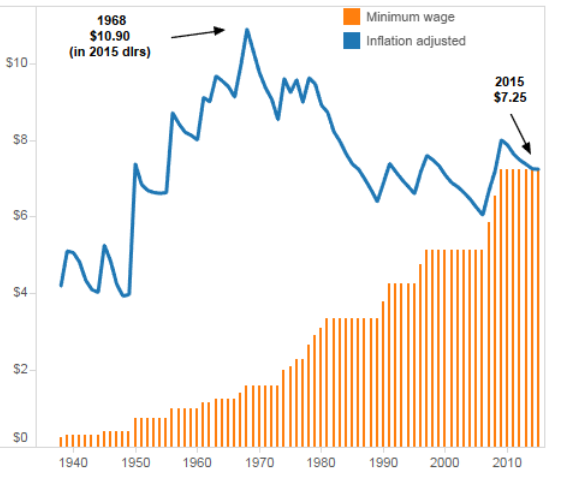
\includegraphics[width=2.8in]{cnbc_graph.png}

\raggedleft
\tiny{Published by CNBC, source: BLS}
\end{frame}


\begin{frame}{This Study}
\begin{itemize}
\item Six contiguous East Coast states increased minimum wage at the start of 2017
\item Variation in minimum wage across states and within states
\item Analyze full menus from two online sources
\item Analyze restaurant specific characteristics 
\begin{itemize}
\item Quality
\item Border effects
\end{itemize}

\end{itemize}
\end{frame}





\begin{frame}[label=main]{Minimum Wage Laws}
\footnotesize
\centering
\begin{tabular}{ c c c c c c c} \\ \hline \hline
&  \multicolumn{3}{c}{Regular Minimum Wage} & \multicolumn{3}{c}{Tipped Minimum Wage}\\
 Area & `16  & `17  & $\% \Delta$ & `16 & `17 &  $\% \Delta$  \\ \hline \hline
 NYC \& FF & \$10.50 & \$12.00 & 14.29\%& - & - & - \\
 NY Upstate \& FF  & \$9.75 & \$10.75 & 10.26\% & - & -& - \\
NYC \& Lg & \$9.00 & \$11.00 & 22.22\% & \$7.50 & \$7.50 & 0.00\%\\
NYC \& Sm & \$9.00 & \$10.50 & 16.67 \% & \$7.50 & \$7.50 & 0.00\%\\
NYC MSA & \$9.00 & \$10.00 & 11.11\% & \$7.50 & \$7.50 & 0.00\%\\
NY Upstate & \$9.00 & \$9.70 & 7.78\% & \$7.50 & \$7.50  & 0.00\% \\
Connecticut & \$9.60 & \$10.10 & 5.21\% & \$6.07 & \$6.38 & 5.11\% \\
New Jersey &  \$8.38 & \$8.44 & 0.72\%  & \$2.13 & \$2.3 & 0.00\% \\
Massachusetts & \$10.00 & \$11.00 & 10.00\% & \$3.00 & \$3.75  & 25.00\% \\
Pennsylvania &  \$7.25 & \$7.25 & 0.00\% & \$2.83 & \$2.83 & 0.00\% \\
Vermont &  \$9.60 & \$10.00 & 4.2\% & \$4.80 & \$5.00 & 4.2\% \\
\end{tabular}
\raggedleft
\hyperlink{supplemental}{\beamerbutton{NY Schedule}}
\end{frame}




\begin{frame}{Minimum Wage Change By County}

\centering
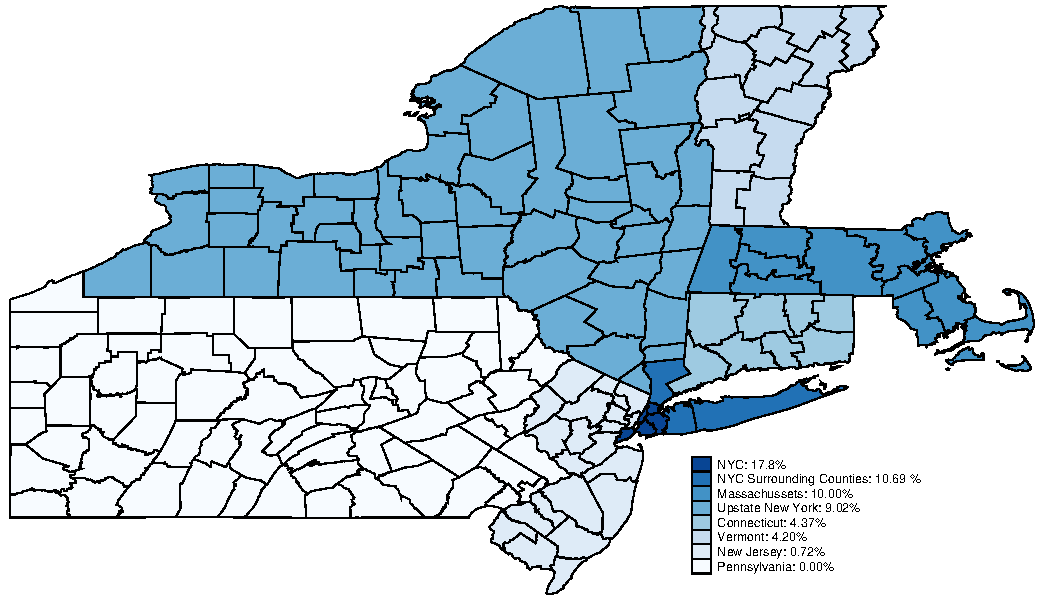
\includegraphics[scale=.65]{counties.pdf}

\end{frame}

\section{Data}

\begin{frame}{Data}
Yelp 
\begin{itemize}
\item Basic restaurant info, item and price info
\item Star rating 
\item Quarterly data: Apr `16, Jul `16, Oct `16, Jan `17, Apr '17
\end{itemize}

Grubhub
\begin{itemize}
\item Basic restaurant info, item and price info
\item Monthly data: Dec `16, Jan `17, Feb `17, Mar `17, Apr '17
\end{itemize}

ReferenceUSA
\begin{itemize}
\item Business data
\item Sales, employees, restaurant type, franchise status
\end{itemize}

\end{frame}




\begin{frame}{Sample of Restaurants}

\centering
\small
\begin{tabular}{ccccccc } \\ \hline \hline
Source & N & \%LS  & \% Chain   & \% Small & Price \\ \hline \hline
&&& \\
RUSA & 89,114 & 19.94 & 14.06 & 75.72 & -\\
\\
Yelp (All) & 35,502 & 17.01 & 11.82 & 75.13& - \\
\\
Yelp (Prices) & 7,901 & 5.49  & 1.77 & 78.40 & 9.37 \\
\\ 
Grubhub  & 5,351 & 6.48 & 2.01 &  86.19 & 8.66 \\
\end{tabular}
\end{frame}

\begin{frame}{Sample Size by Min Wage Group}
\scriptsize
\centering
\begin{tabular}{c c c c c c } \\ \hline \hline
Area & \% Increase & Yelp Restaurants   & Grubhub Restaurants\\ \hline \hline
&&& \\
 NYC \& FF  & 14.29\% & 25   & 34 \\
 NY Upstate \& FF  & 10.26\% & 3&13 \\
NYC \& Lg & 22.22\% & 610 &  407\\
NYC \& Sm & 16.67 \% & 2,408 &  2,266\\
NYC MSA & 11.11\% & 425 &341\\
NY Upstate & 7.78\% & 378 &  207 \\
Connecticut & 5.21\% & 57  &  93 \\
New Jersey & 0.72\% & 1,479 & 792\\
Massachusetts & 10.00\% & 1,391 &  550\\
Pennsylvania & 0.00\% &  1,072 &  647\\
Vermont & 4.2\% & 50 & 2\\
\\ \hline
Total & & 7,901 &  5,351 \\
\end{tabular}
\end{frame}


\begin{frame}{Sample of Yelp Restaurants}

\centering
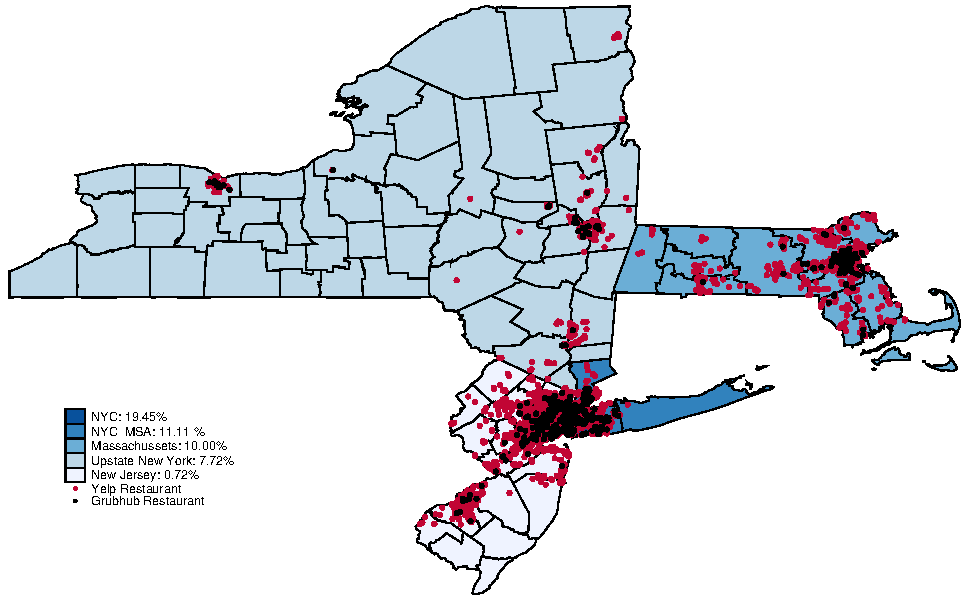
\includegraphics[scale=.65]{map_yelp.pdf}

\end{frame}

\section{Price Pass Through}

\begin{frame}{Expected Price Pass Through}
Assumptions:
\begin{itemize}
\item Factor markets competitive
\item Product monopolistically competitive
\item Firms have constant returns to scale production function
\end{itemize}

\bigskip

Price Pass Through:

\bigskip
\centering{($\% \Uparrow$ MW) $x$  ($\frac{MW Costs}{Labor Costs}$)  $x$  ($\frac{Labor Costs}{Total Costs}$) }

\bigskip
\centering{ (10\%) $x$ (17-33\%) $x$ (33\%) = 0.56-1.09\%}

\end{frame}

\begin{frame} {Model of Price Pass Through}

\begin{dmath}
\Delta \ln p_{ijkt} = \sum_{h=0}^{2}\beta_h \Delta \ln mw_{kt-h} +  \gamma \Delta \ln p_{ijkt-1}  + \boldsymbol{X}_j \boldsymbol{\lambda} + \epsilon_k + \epsilon_t + \epsilon_{ijkt}
\end{dmath}

$i$ = item

$j$ = restaurant

$k$ = minimum wage group

$t$ = observation period

$\boldsymbol{X}_j$= vector of covariates: chain, LS, employees, sales, total items

\end{frame}




\begin{frame}{Price Pass Through of a 10\% MW Increase}
\centering
\scriptsize
{
\def\sym#1{\ifmmode^{#1}\else\(^{#1}\)\fi}
\begin{tabular}{l*{4}{c}}
\hline\hline
                    &\multicolumn{1}{c}{(1)}&\multicolumn{1}{c}{(2)}&\multicolumn{1}{c}{(3)}&\multicolumn{1}{c}{(4)}\\
                    &\multicolumn{1}{c}{Yelp}&\multicolumn{1}{c}{Yelp}&\multicolumn{1}{c}{GH}&\multicolumn{1}{c}{GH}\\
\hline
$ Oct - Jan  $&      0.0707\sym{*}  &      0.0708\sym{**} &       &      \\
                    &    (0.0309)         &    (0.0291)         &           &    \\
[1em]
$ Dec - Jan $&      &       &       0.140\sym{***}&       0.165\sym{***}\\
                    &          &         &    (0.0135)         &    (0.0141)         \\
[1em]
$ Jan - Feb $&                     &                     &       0.219\sym{**} &       0.244\sym{**} \\
                    &                     &                     &    (0.0595)         &    (0.0607)         \\
 [1em]
$Feb - March$&                     &                     &       0.255\sym{**} &       0.280\sym{**} \\
                    &                     &                     &    (0.0632)         &    (0.0700)         \\
\hline
Total Pass Through & 0.071 & 0.071 & 0.614 & 0.689 \\
Controls & No & Yes & No & Yes \\
Observations        &     1571872         &     1571872         &     1465718         &     1465718         \\
\hline\hline
\multicolumn{5}{l}{\footnotesize Standard errors in parentheses}\\
\multicolumn{5}{l}{\footnotesize \sym{*} \(p<.10\), \sym{**} \(p<.05\), \sym{***} \(p<.001\)}\\
\end{tabular}
}

\end{frame}





\begin{frame}{Price Pass Through By Item Type \\ \small{Grubhub}}
\centering
\tiny
{
\def\sym#1{\ifmmode^{#1}\else\(^{#1}\)\fi}
\begin{tabular}{l*{7}{c}}
\hline\hline
                    &\multicolumn{1}{c}{(1)}&\multicolumn{1}{c}{(2)}&\multicolumn{1}{c}{(3)}&\multicolumn{1}{c}{(4)}&\multicolumn{1}{c}{(5)}&\multicolumn{1}{c}{(6)}&\multicolumn{1}{c}{(7)}\\
                    &\multicolumn{1}{c}{Popular}&\multicolumn{1}{c}{Side}&\multicolumn{1}{c}{Sandwich}&\multicolumn{1}{c}{Pizza}&\multicolumn{1}{c}{Entre}&\multicolumn{1}{c}{Desert}&\multicolumn{1}{c}{Drink}\\
\hline
$Dec - Jan$&       0.142\sym{**} &      0.0997\sym{**} &       0.313\sym{***}&       0.213\sym{**} &       0.218\sym{***}&      0.0877         &       0.101\sym{**} \\
                    &    (0.0463)         &    (0.0294)         &   (0.00973)         &    (0.0689)         &    (0.0108)         &    (0.0498)         &    (0.0347)         \\
[1em]
$Jan - Feb$&       0.550\sym{**} &      0.0878\sym{**} &       0.354\sym{**} &       0.326\sym{**} &       0.233\sym{***}&       0.167\sym{**} &       0.413\sym{**} \\
                    &     (0.218)         &    (0.0243)         &    (0.0790)         &     (0.103)         &    (0.0285)         &    (0.0653)         &     (0.110)         \\
[1em]
$Feb - Mar$&       0.492\sym{*}  &       0.210\sym{**} &       0.434\sym{**} &       0.325\sym{**} &       0.213\sym{**} &       0.241\sym{*}  &       0.362\sym{*}  \\
                    &     (0.227)         &    (0.0416)         &    (0.0850)         &    (0.0624)         &    (0.0659)         &     (0.126)         &     (0.169)         \\
\hline
Total & 1.184 & 0.397 & 1.101 & 0.864 & 0.664 & 0.496 & 0.876 \\
Observations        &       86259         &      172901         &      201821         &       70966         &      270068         &       33805         &      111161         \\
\hline\hline
\multicolumn{8}{l}{\footnotesize Standard errors in parentheses}\\
\multicolumn{8}{l}{\footnotesize \sym{*} \(p<.10\), \sym{**} \(p<.05\), \sym{***} \(p<.001\)}\\
\end{tabular}
}

\end{frame}





\section{Quality}






\begin{frame}{Min Wage Impact on Yelp Star Ratings}

\begin{dmath}
\Delta \ln(exact\_stars_{jkt}) =\beta \ln mw_{kt-h}  +    \gamma stars\_apr16_{jkt} +\boldsymbol{X}_j  \boldsymbol{\lambda} + \epsilon_k + \epsilon_t + \epsilon_{ijkt}
\end{dmath}

$exact\_stars_{jkt}$: average star rating to the tenth

$stars\_apr16_{jkt}$: rounded average star rating


\end{frame}


\begin{frame}{Min Wage Impact on Yelp Star Ratings}
\centering
\scriptsize
<<<<<<< HEAD
\begin{center}
\begin{tabular}{lcccccc}
\hline  & (1) & (2) & (3) & (4) & (5) & (6)\\
 & All &  $ 2.5 $  &  $ 3.0 $  &  $ 3.5 $  &  $ 4.0 $  &  $ 4.5$ \\
\hline  $ Apr16-Jul16 $  & 0.035 & 1.138 & 0.625 & 0.068 & -1.047 & -0.627\\
 & (0.213) & (1.201) & (0.697) & (0.187) & (0.312) & (0.456)\\
 $ Jul16-Oct16 $  & -0.046 & -0.321 & -0.305 & 0.109 & 0.198 & -0.792\\
 & (0.071) & (0.292) & (0.400) & (0.211) & (0.296) & (0.413)\\
 $ Oct16-Jan17 $  & 0.049 & 0.255 & -1.341 & -0.268 & 0.500 & 0.470\\
 & (0.036) & (1.068) & (0.178) & (0.076) & (0.090) & (0.275)\\
 $ Jan17-Apr17 $  & -0.416 & -1.158 & -0.546 & -0.728 & -0.252 & -0.255\\
 & (0.167) & (0.609) & (0.670) & (0.197) & (0.080) & (0.175)\\
\hline \textit{Total \% Change Stars} & -0.368 & -0.903 & -1.887 & -0.996 & 0.248 & 0.215\\
  & (0.138) & (1.667) & (0.813) & (0.161) & (0.123) & (0.164)\\
\hline  $ N $  & 6392 & 625 & 1080 & 1801 & 1904 & 982\\
 $ NxT $  & 25568 & 2500 & 4320 & 7204 & 7616 & 3928\\
\hline\end{tabular}\\
\begin{tiny} \hfil\end{tiny}\\
\end{center}
=======
\begin{center}
\begin{tabular}{lcccccc}
\hline  & (1) & (2) & (3) & (4) & (5) & (6)\\
 & All &  $ 2.5 $  &  $ 3.0 $  &  $ 3.5 $  &  $ 4.0 $  &  $ 4.5$ \\
\hline  $ Apr16-Jul16 $  & 0.035 & 1.138 & 0.625 & 0.068 & -1.047 & -0.627\\
 & (0.213) & (1.201) & (0.697) & (0.187) & (0.312) & (0.456)\\
 $ Jul16-Oct16 $  & -0.046 & -0.321 & -0.305 & 0.109 & 0.198 & -0.792\\
 & (0.071) & (0.292) & (0.400) & (0.211) & (0.296) & (0.413)\\
 $ Oct16-Jan17 $  & 0.049 & 0.255 & -1.341 & -0.268 & 0.500 & 0.470\\
 & (0.036) & (1.068) & (0.178) & (0.076) & (0.090) & (0.275)\\
 $ Jan17-Apr17 $  & -0.416 & -1.158 & -0.546 & -0.728 & -0.252 & -0.255\\
 & (0.167) & (0.609) & (0.670) & (0.197) & (0.080) & (0.175)\\
\hline \textit{Total \% Change Stars} & -0.368 & -0.903 & -1.887 & -0.996 & 0.248 & 0.215\\
  & (0.138) & (1.667) & (0.813) & (0.161) & (0.123) & (0.164)\\
\hline  $ N $  & 6392 & 625 & 1080 & 1801 & 1904 & 982\\
 $ NxT $  & 25568 & 2500 & 4320 & 7204 & 7616 & 3928\\
\hline\end{tabular}\\
\begin{tiny} \hfil\end{tiny}\\
\end{center}
>>>>>>> 9bf80c4d3367c601bceb3268e37dc31cf9116a6c

\end{frame}



\section{Border Effects}

\begin{frame}{Border Effects}
\centering
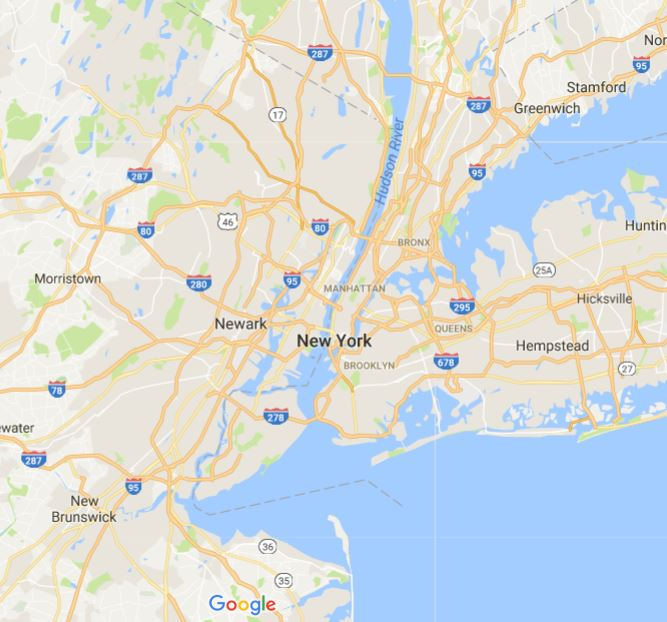
\includegraphics[width=2.8in]{nynj_map_google.jpg}

\end{frame}

\begin{frame}{Border Effects}

$$
\begin{aligned}
\Delta \ln (p_{ij,Oct-Feb})  = & \alpha_0 + \alpha_1  \mathbbm{1}(NY=1)  \\
& + \alpha_2 D_{j} + \alpha_3[D_j * \mathbbm{1}(NY=1)]  \\
& +\gamma X_{ij}  + \epsilon_{ij} 
\end{aligned}
$$

$D_j$: minutes to a competitor across the border

$\mathbbm{1}(NY=1)$: indicator function for state

\bigskip

\begin{centering}

NY: $
\Delta \ln (p_{ij,Oct-Feb})  = (\alpha_0 +\alpha_1) +  (\alpha_2 + \alpha_3) D_j +\gamma X_{ij}  + \epsilon_{ij}   
$

\bigskip

NJ:
$
\Delta \ln (p_{ij,Oct-Feb})  = (\alpha_0 ) +  (\alpha_2 ) D_j +\gamma X_{ij}  + \epsilon_{ij}   
$

\end{centering}
\end{frame}

\begin{frame}{Border Effects}

\centering
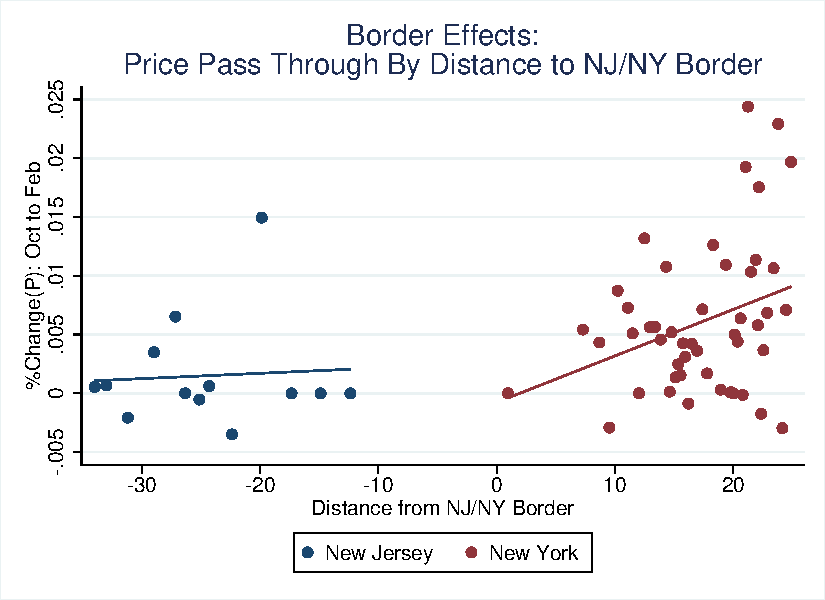
\includegraphics[width=4in]{total_pricechange_dist_nynj.pdf}
\end{frame}

\begin{frame}{Border Effects: Results}
\centering
\tiny
{
\def\sym#1{\ifmmode^{#1}\else\(^{#1}\)\fi}
\begin{tabular}{l*{4}{c}}
\hline\hline
                    &\multicolumn{1}{c}{(NJ)}&\multicolumn{1}{c}{(NJ)}&\multicolumn{1}{c}{(NJ)}&\multicolumn{1}{c}{(NY MSA)}\\
                    &\multicolumn{1}{c}{$\Delta Ln(P_{feb-oct})$}&\multicolumn{1}{c}{$\Delta Ln(P_{feb-oct})$}&\multicolumn{1}{c}{$\Delta Ln(P_{oct-jul})$}&\multicolumn{1}{c}{$\Delta Ln(P_{feb-oct})$}\\
\hline
Constant ($ \alpha_0 $)           &     0.00261         &     0.00268         &   -0.000689         &     0.00198         \\
                    &   (0.00145)         &   (0.00146)         &  (0.000873)         &   (0.00318)        \\
        [1em]
NYC ($ \alpha_1 $)     &    -0.00339\sym{*}  &    -0.00410\sym{*}  &     0.00218\sym{*}  &       -0.00589              \\
                    &   (0.00160)         &   (0.00161)         &  (0.000961)         &                     (0.00329)   \\
[1em]
Distance   ($\alpha_2$)            &   0.0000454         &   0.0000683         &  -0.0000366         &                      0.000245         \\
                    & (0.0000566)         & (0.0000568)         & (0.0000339)         &                     (0.000168)      \\
%[1em]
%ny=0 $\times$ dist\_nynj\_bord&           0         &           0         &           0         &                     \\
%                    &         (.)         &         (.)         &         (.)         &                     \\
[1em]
NYC $\times$ Distance ($\alpha_3$)    &    0.000350\sym{***}&    0.000322\sym{***}&   0.0000461         &     0.000293                 \\
                    & (0.0000678)         & (0.0000679)         & (0.0000405)         &                     (0.000177)   \\
%Chain               &                     &    -0.00553\sym{*}  &    -0.00222         &                     \\
%                    &                     &   (0.00243)         &   (0.00145)         &                     \\
%[1em]
%LS                  &                     &    -0.00383\sym{***}&    -0.00113\sym{*}  &                     \\
%                    &                     &  (0.000907)         &  (0.000542)         &                     \\
%[1em]
%Employees           &                     &  -0.0000586         &   0.0000367         &                     \\
%                    &                     & (0.0000472)         & (0.0000282)         &                     \\
%[1em]
%Sales               &                     &    2.48e-09\sym{***}&    1.82e-11         &                     \\
%                    &                     &  (4.42e-10)         &  (2.64e-10)         &                     \\
%[1em]
%nyc                 &                     &                     &                     &    -0.00589         \\
%                    &                     &                     &                     &   (0.00329)         \\
%[1em]
%dist\_nyny\_bord      &                     &                     &                     &    0.000245         \\
%                    &                     &                     &                     &  (0.000168)         \\
%[1em]
%nyc=0 $\times$ dist\_nyny\_bord&                     &                     &                     &           0         \\
%                    &                     &                     &                     &         (.)         \\
%[1em]
%nyc=1 $\times$ dist\_nyny\_bord&                     &                     &                     &    0.000293         \\
%                    &                     &                     &                     &  (0.000177)         \\
%[1em]
 \\
\hline
Observations        &       80402         &       80402         &       80402         &       23368         \\
\hline\hline
%	\multicolumn{5}{l}{\footnotesize Standard errors in parentheses}\\
%	\multicolumn{5}{l}{\footnotesize \sym{*} \(p<0.05\), \sym{**} \(p<0.01\), \sym{***} \(p<0.001\)}\\
\end{tabular}
}


\end{frame}

\begin{frame}{Border Effects: Interpretation}
For restaurants in NYC within 20 minutes of the NJ border...
\begin{itemize}
\item On average, a 1 minute increase in the distance from the NJ border \\ $\Rightarrow$ .03 percentage point increase in $\%\Delta$ price 
\item On average, a 10 minute increase in the distance from the NJ border \\ $\Rightarrow$ .3 percentage point increase in $\%\Delta$ price 
\end{itemize}
Av$(\%\Delta(p))$ for all items in NYC from Oct to Feb = 0.80

\end{frame}

\section{Conclusion}

\begin{frame}{Conclusion}
 How do restaurant prices change in response to increases in the minimum wage?
\begin{itemize}
\item Significant price pass through consistent with literature
\item Heterogeneity across restaurant characteristics
\item Heterogeneity across item type
\end{itemize}
 How is customer perceived quality of restaurants affected by a minimum wage increase?
\begin{itemize}
\item Good restaurants get better
\item Bad restaurants get worse
\end{itemize}
 Do border effects have an impact on price pass through?
\begin{itemize}
\item Yes, in areas with a minimum wage increase
\end{itemize}
\end{frame}


\begin{frame}[label=supplemental]{Minimum Wage Laws: Fight for 15 Schedule}
\footnotesize
\centering
\begin{tabular}{ c c c c c c c} \\ \hline \hline
 Area & 201 7& 2018 & 2019 & 2020 & 2021 & 2022 \\ \hline \hline
 NYC \& FF & \$12.00 & \$13.50 & \$15.00 \\
 NY Upstate \& FF  & \$10.75 & \$11.75 & \$12.75 & \$13.75 & \$15.00 \\
NYC \& Lg & \$11.00 & \$13.00 & \$15.00 \\
NYC \& Sm & \$10.50 & \$12.00 & \$13.50 & \$15.00 \\
NYC MSA & \$10.00 & \$11.00 & \$12.00 & \$13.00 & \$14.00 &  \$15.00 \\
NY Upstate &\$9.70 & \$10.40 & \$11.10 &  \$11.80 & \$12.50 & ... \\
%Connecticut & \$10.10  \\
%New Jersey & \$8.44  \\
%Massachusetts &  \$11.00 \\
%Pennsylvania & \$7.25 \\
%Vermont & \$10.00 & \$10.50  \\
\end{tabular}

\bigskip

\raggedleft
\hyperlink{main}{\beamerbutton{Back}}
\end{frame}


\end{spacing}
\end{document}











































